\section{Dominoes}

(Partial) lock rule? Constructible configurations. 

\subsection{Tetris with vertical dominoes}

Using the introduced notation, the problem is $\textsc{Tetris-NoRotation}\lbrack \VD \rbrack $ both  \clearing and \survival. The input consist of sequence of vertical dominoes and an arbitrary sized $n \times m$ board in a contractible configuration. The initial state function used in this variation differs since the default on the initial orientation, since the pieces must come in vertical orientation.

\subsubsection{Constructible board configurations}

First we will to characterize the constructible boards with $\VD$ pieces without rotation by exploring the configuration starting from an empty board. Vertical dominoes consist of two vertical adjacent cells. 

For an empty board, any trajectory fixes the piece in the bottom row, filling $\cell[1][i]$ and $\cell[2][i]$ cells for any $1 \leq i \leq m$. The next domino can either go to an empty column or to the one before. Placing the first $m$ dominoes in unfilled columns clears the two lowest rows, and consequently the board. When a domino is placed in a non-empty column $i$, the $\cell[3][i]$ and $\cell[4][i]$ are filled, and so on, util a $\VD$ is placed in the last unfilled column. When this happens the two lowest rows are cleared and the process continues. 

So we can represent a reachable configuration of a given $n \times m$ board $B$ with a sequence of $m$ integers $(a_1, \dots, a_m)$, where

$$0 \leq a_i \leq \lceil \frac{n}{2} \rceil, \;\;\;   \forall i = 1,\dots, m$$

and $\exists i$ such that $a_i = 0$ (an empty column), with the following mapping: 

$$
\cell = \begin{cases}
   \text{filled}  & \text{if } i \leq  2a_j  \\
   \text{empty}   & \text{if } i >  2a_j
\end{cases}
$$

Each $a_i$ counts the number of vertical pieces placed in the column $i$. For example, in a $10 \times 6 $  board, the sequence $(1,2,0,4,2,3)$ defines the configuration in 
\ref{dom:vconf}.

\begin{figure}[h]
    \centering
    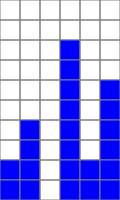
\includegraphics[width=0.2\textwidth]{./pictures/dominoes/vertical_configuration.pdf}
    \caption{The $10 \times 6 $ board configuration represented by the sequence $(1,2,0,4,2,3)$.}
    \label{dom:vconf} 
\end{figure}

\subsubsection{Cleaing}

In this decisional problem the input is a sequence of $k$ vertical dominoes and an $n \times m$ board with an initial configuration, that can be represented by the sequence $(a_1, \dots, a_m)$ as before. The question is: \emph{Is ther a way to clean the board after placing the $k$ pieces?}

\begin{theorem} 
$\textsc{Tetris-NoRotation}\lbrack \VD \rbrack $ \clearing is in \pp.
\label{dom:no-rot-vd}
\end{theorem}
\begin{proof}
    Let $B = (a_1, \dots, a_m) $ be the board representation and $k$ the length of the sequence of vertical dominoes. For every constructible board there is an empty column, so the strategy consists on placing each piece in an arbitrary empty column. 

    All the empty cells under the lowest empty row need to be filled to clean the board. Let $a_{\max}$ be the max in the board representation. Since we fill cells with dominoes, the number of dominoes $k_{\min}$ needed to clean the board is:
    $$ k_{\min} = \sum_{i = 1}^m \left( a_{\max} - a_i \right) $$

    If $k < k_{\min}$ we can't clear the board. If $k =  k_{\min}$ we can clear the board. And when $k > k_{\min}$, we can clean the board if after placing $k_{\min}$ dominoes the number of remaining pieces is a multiple of the board width, $k - k_{\min} \equiv 0 \mod m$. Since all the computations can be done in polyatomic time in respect of the input, the problem is in \pp.
\end{proof}

For boards with an even number of rows all pieces always fit inside the board. For an odd number of rows, dominoes could be placed in the top row with half of the domino inside the board and half outside. If we allow this, by changing the \emph{fix} function, the result would be the same since the same strategy works. The Figure~\ref{dom:vconf-filled} shows, in yellow color, how the number of pieces needed to clean the board are counted in Figure~\ref{dom:vconf}

\begin{figure}[h]
    \centering
    \includegraphics[width=0.2\textwidth]{./pictures/dominoes/vertical_configuration_filled.pdf}
    \caption{The $10 \times 6 $ board configuration needs 13 dominoes to be cleared.}
\label{dom:vconf-filled} 
\end{figure}


\subsubsection{Survival}

With the same input, the objective is to do not lose. The last proof provides a strategy to survive indefinitely. So for any number of pieces $k$ there is a way to avoid losing. Hence:
\begin{theorem} 
$\textsc{Tetris-NoRotation}\lbrack \VD \rbrack $ \survival is in \pp.
\end{theorem}


\subsection{Tetris with vertical dominoes}

As before, the problem is $\textsc{Tetris-NoRotation}\lbrack \HD \rbrack $ both \clearing and \survival. Placing a horizontal domino fills two adjacent cells in one row or clears the row. In any construtible board, each row has an even number of filled cells. When the board width is odd no row can be cleared, because to clear a row all the cells have to be filled. In this scenario the board can be cleared if the input consists on an empty board and an empty sequence of pieces. 

From now and on we assume the board has an even number of columns. Let $B$ be a board with $c$ columns. Let's divide the board in $c/2$ \emph{buckets}, a pair of consecutive columns. Then:

\begin{lemma0}   
    Not placing a domino inside a bucket makes the row unclearable.
\end{lemma0}
\begin{proof}
    Let $r$ be a row containing some dominoes. When a domino is placed in a bucket it divides the row into two parts: the cells on the left side of the domino and the ones on the right. Both parts of even length, and containing an even number of filled cells.

    In the other case the two parts have an odd length but containing an eaven number of filled cells, making them impossible to clean
    since there's no way to add an odd number of cells by placing dominoes.
\end{proof}

For example, in the Figure~\ref{dom:buckets}, the second piece occupies the second and the third bucket, making the row un-clearable. 

\begin{figure}[h]
    \centering
    \includegraphics[width=0.2\textwidth]{./pictures/dominoes/buckets.pdf}
    \caption{A board with one partially filled row.}
    \label{dom:buckets} 
\end{figure}

We now can prove both clearing and survival problems.

\begin{theorem}
    $\textsc{Tetris-NoRotation}\lbrack \HD \rbrack $ \clearing is in \pp.
\end{theorem}
\begin{proof}


    The input is an $n \times m$ input board $B$, filled with a construable configuration, and sequence of $k$ dominoes $\HD$. If $m$ is odd then the board can't be cleared if $k > 0$ or the initial board isn't empty. 

    When $m$ is even we first need to check if the board is clearable. If there's only one row, checking that the row has been built by placing each piece inside a bucket determines if the row is clearable. When the board has more than one row the same happens. 

    We first group in pieces the filled cells of each row from the initial board. This can always be done because there's no way to clean \emph{"half"} piece. Then we check if each piece is placed inside a bucket. If any piece isn't placed inside a bucket the board can't be cleared. We can compute this in $\mathcal{O}(n\cdot m)$.

    Now the board can be represented with a sequence $(a_1, \dots, a_{m/2})$ of $m/2$ numbers each representing the number of dominoes placed in each bucket. Let $a_{\max}$ be the maximum of the sequence. The minimum number of pieces needed to clear the board is:

    $$ k_{\min} = \sum_{i = 1}^{m/2} (a_{\max} - a_i )$$

    If $k < k_{\min}$ the board can't be cleared. If $k = k_{\min}$ the board can be cleard. When $k > k_{\min}$ the board can be cleared if $ k - k_{\min} \equiv 0 \mod m / 2$, we must ensure the remaining pieces to leave the board empty by filling rows.
\end{proof}

\begin{figure}[ht]
  \centering
  \begin{subfigure}[b]{0.3\textwidth}
    \centering
    \includegraphics[width=0.9\textwidth]{pictures/dominoes/horitzonatl_configuration_1.pdf}
    \caption{}
  \end{subfigure}
  \begin{subfigure}[b]{0.3\textwidth}
    \centering
    \includegraphics[width=0.9\textwidth]{pictures/dominoes/horitzonatl_configuration_2.pdf}
    \caption{}
  \end{subfigure}
  \begin{subfigure}[b]{0.3\textwidth}
    \centering
    \includegraphics[width=0.9\textwidth]{pictures/dominoes/horitzonatl_configuration_3.pdf}
    \caption{}
  \end{subfigure}
  \caption{Some board configurations. In (a) the board can't be cleared because the topmost domino is placed between the first and the second bucket. In (b) the board is represented by the sequence $(2,4,1,0,3)$, it can be cleared. The minimum number of pieces to clean the board is 10, this pieces apear in yellow in (c).}
  \label{dom:horitzonatl_configuration}
\end{figure}

Figure~\ref{dom:horitzonatl_configuration} shows some examples.

\begin{theorem}
    $ \textsc{Tetris-NoRotation}\lbrack \HD \rbrack $ \survival is in \pp.
\end{theorem}
\begin{proof}
    
    With the given board, we first find (???alortime???) a row to clear. If we find such a row we can survive indefinitely by repeatedly placing pieces in this row.

    If such a row doesn't exists, some dominoes can be placed inside board before a loss. To compute the maximum $k_{min}$(????)...

    If the input length is less or equal than $k_min$ we can survive, if not we can't.

\end{proof}
